\startappendix{Additional Information}
\label{chapter:appendix}

\section{Examples of Methods on Synthetic Data}
  \begin{figure}[!h]
 \centering
 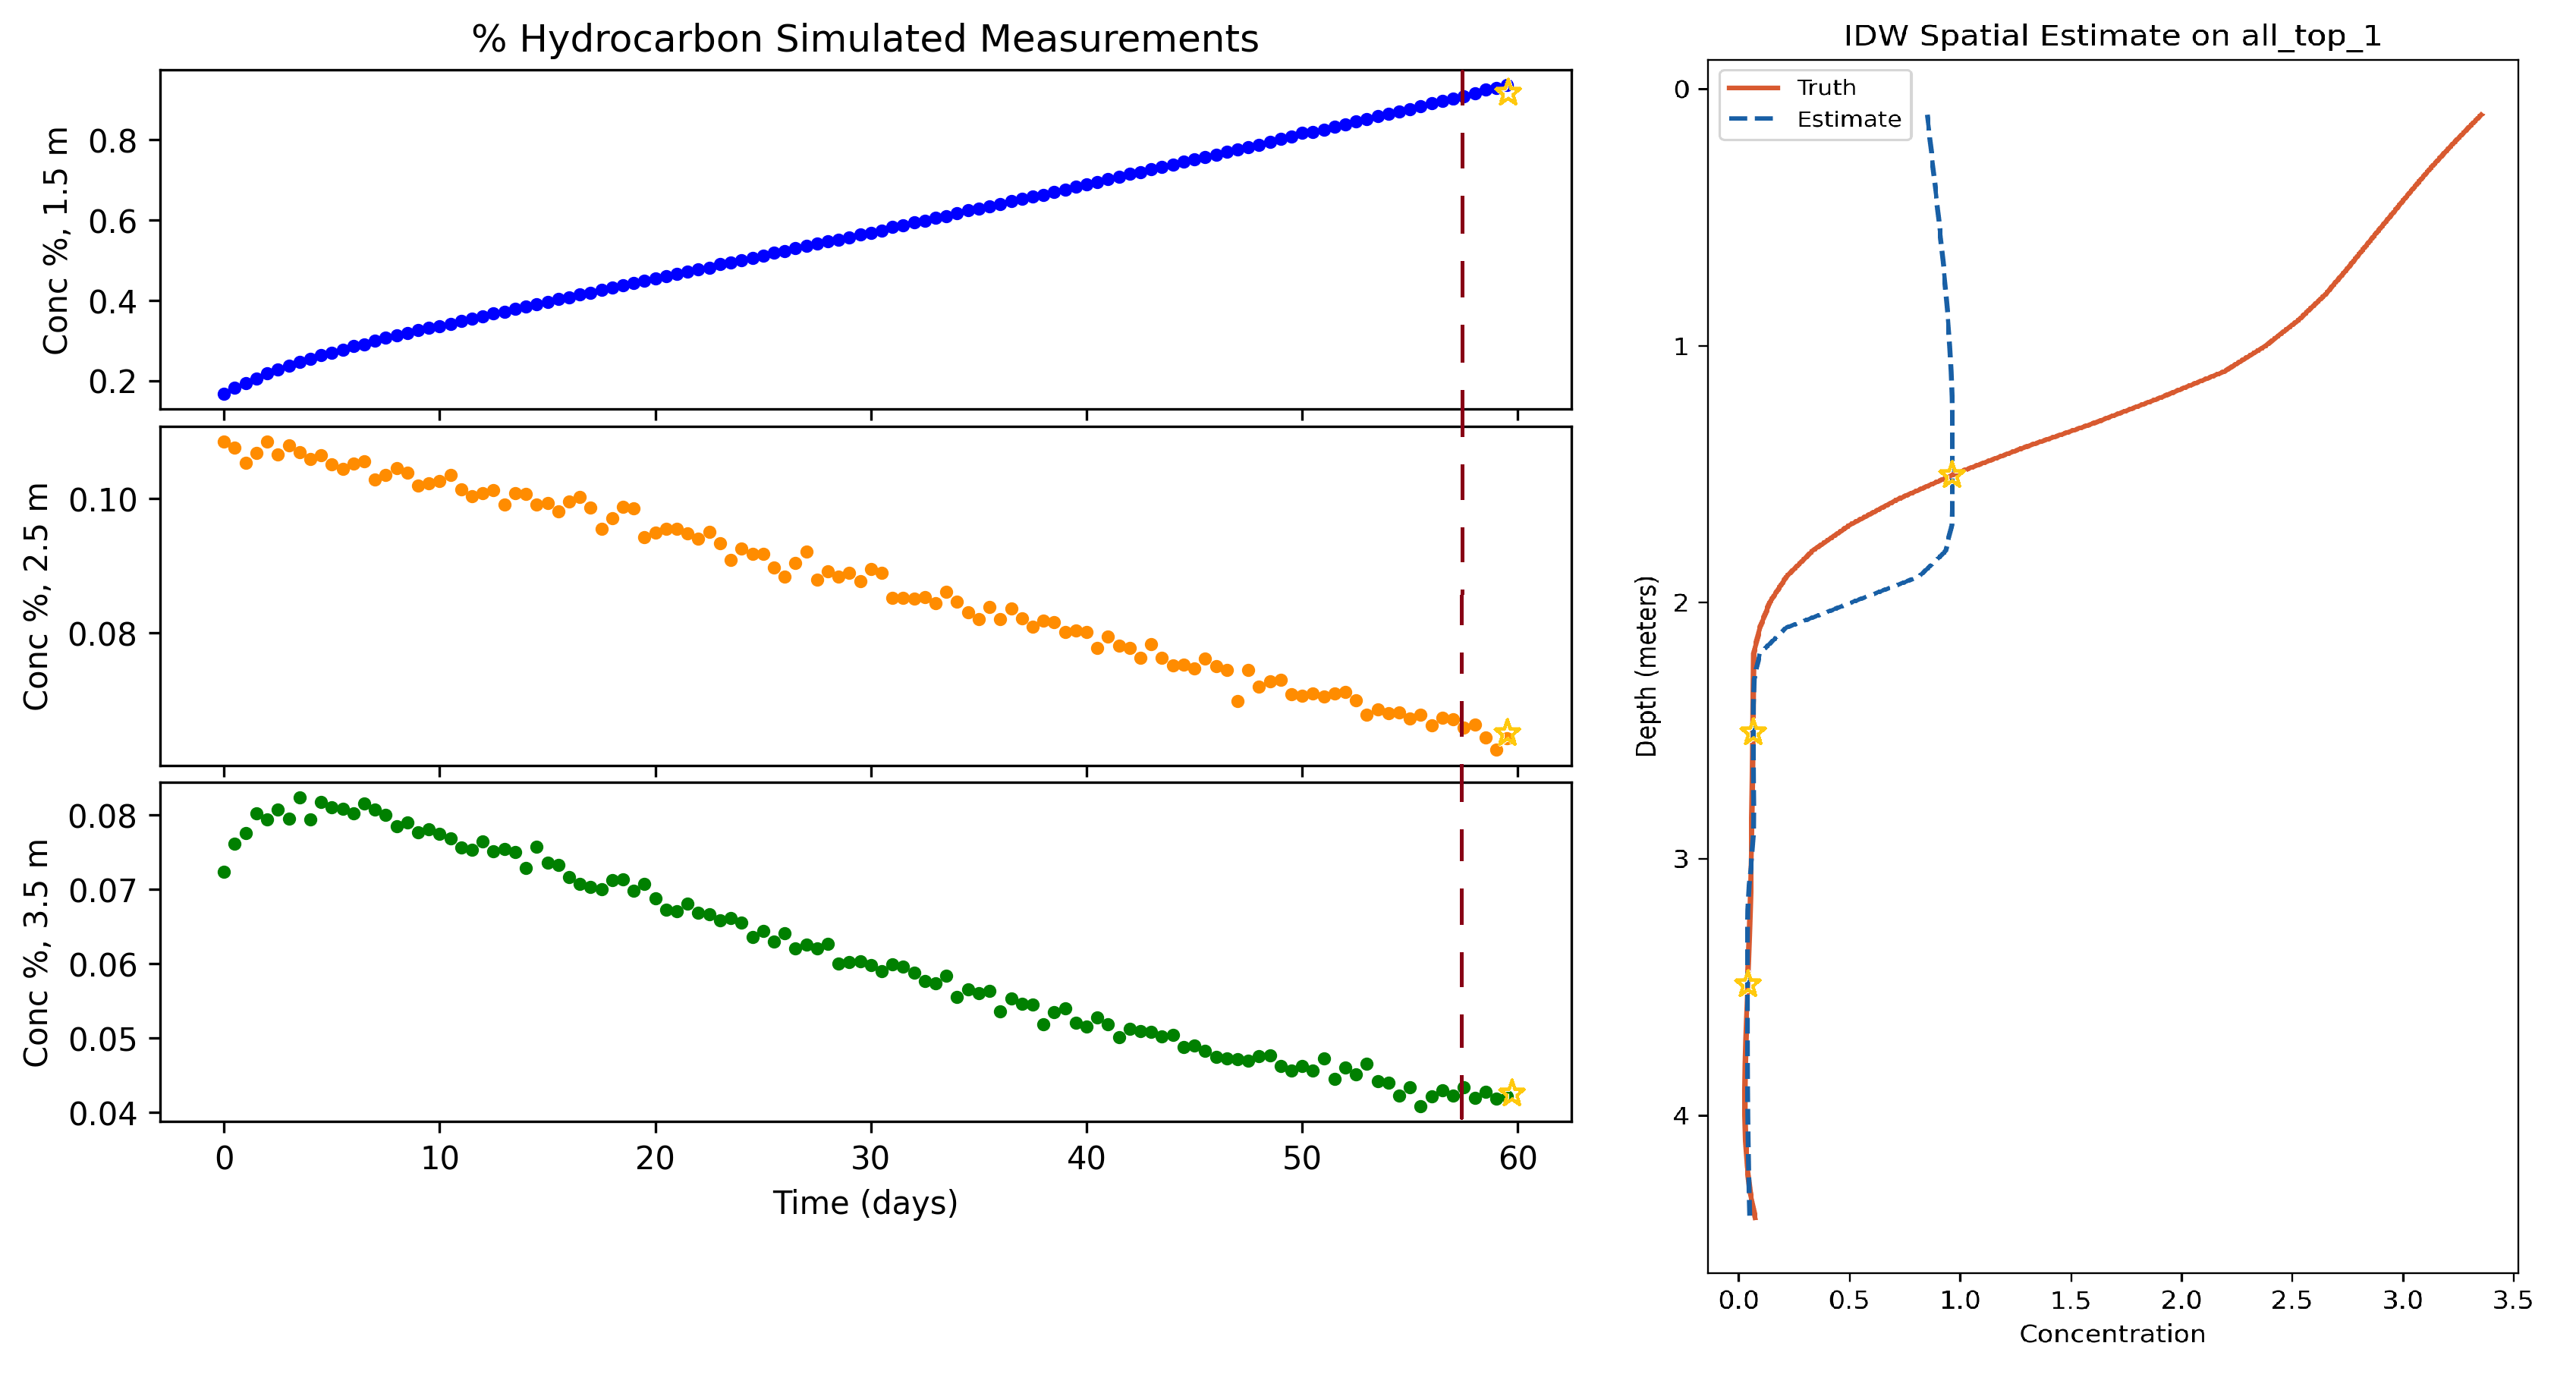
\includegraphics[width = 7in]{figures/idw_temporal_example.png}
 \caption{Example of IDW working on a data sample. The IDW algorithm averages all the measurements in the averaging window depicted by the red line in A. The values are then fed into the IDW algorithm to create the spatial estimate depicted by the blue line in B. This IDW methods uses a power of 4 and an averaging window of 3.}
 \label{fig:idw_example}
 \end{figure} 



  \begin{figure}[!h]
 \centering
 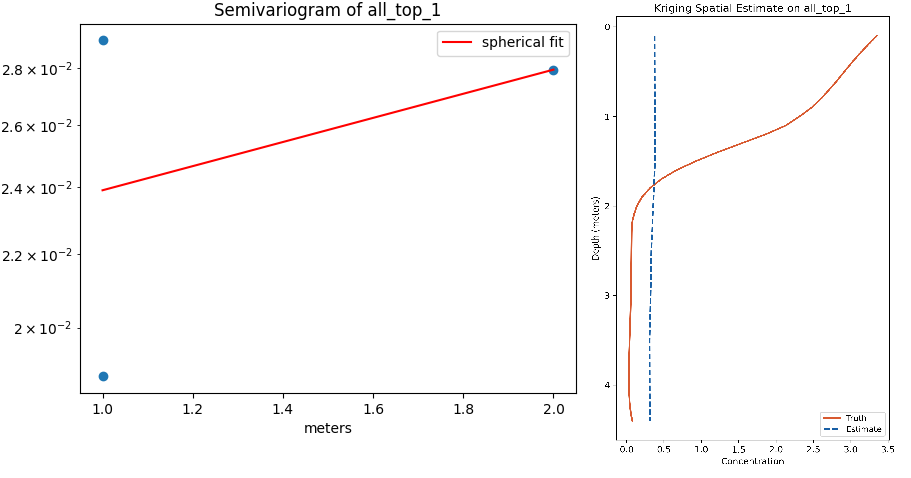
\includegraphics[width = 7in]{figures/kriging_example.png}
 \caption{Example of Kriging on a synthetic data sample. The variogram points are fit with a spherical model. Then the fitted spherical model produces semi-variances to unmeasured points. These semi variances are used as weights in the weighted sum of the measurements. }
 \label{fig:krig_example}
 \end{figure} 


  \begin{figure}[!h]
 \centering
 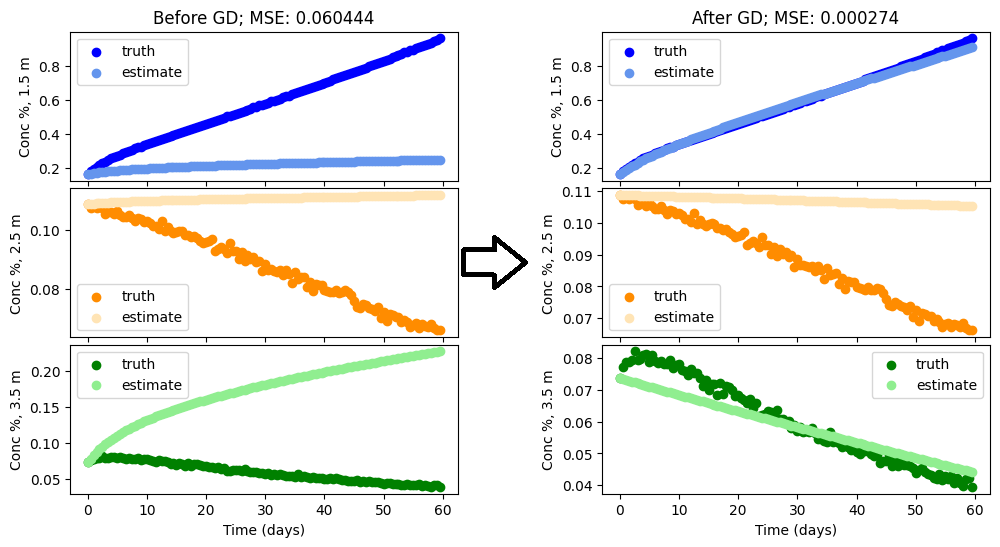
\includegraphics[width = 6.5in]{figures/fdvar_opt_transform.png}
 \caption{The before and after of the optimization process of the 4D-Var. Given the showed measurements, 4D-Var matches a physics-based model. This is the same process for all of the parameter estimation values.}
 \label{fig:fdvar_temporal_example}
 \end{figure} 

 \begin{figure}[!h]
    \centering
    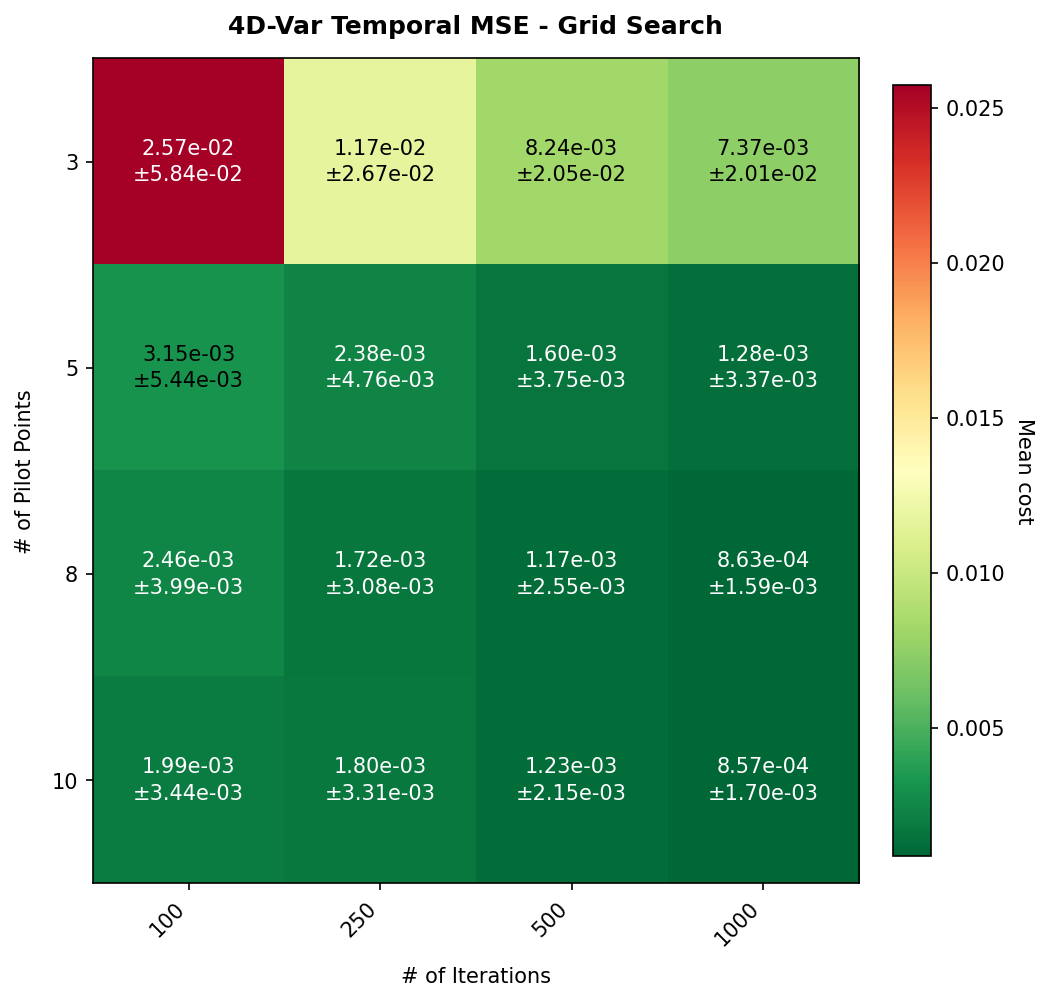
\includegraphics[width=5in]{figures/fdvar_temp_gridsearch_means.png}
    \caption{Hyperparameter grid search of the number of iterations and the number of pilot points for the 4D-Var method. Temporal error comparing $\meas$ and $\est$ after the data has been fit}
    \label{fig:fdvar_temp_gridsearch}
\end{figure}
